\EnableTitleSlide
\section{Aufbau \& Entwicklung \\ der Anwendung}

\begin{frame}{egg}
    \begin{columns}[c]
        \column{.7\textwidth}
            \begin{itemize}
                \item \textbf{egg}: \textbf{e}-\textbf{g}raphs \textbf{g}ood (\url{https://egraphs-good.github.io/})
                \item Bibliothek in Rust zur Erstellung von E-Graphs
                \item \textbf{Paper}: Willsey u.a. 2021 (\url{https://doi.org/10.1145/3434304})
            \end{itemize}\hspace{2.5cm}
        \column{.3\textwidth}
            
\includegraphics[scale=1.9]{utils/egg.pdf}
    \end{columns}
\end{frame}

\begin{frame}{Anwendung (1)}
    
\end{frame}

\begin{frame}{Anwendung (2)}
    
\end{frame}

\begin{frame}{Anwendung (3)}
    
\end{frame}

\begin{frame}{Aufbau}
    \begin{figure}[H]
        \centering
        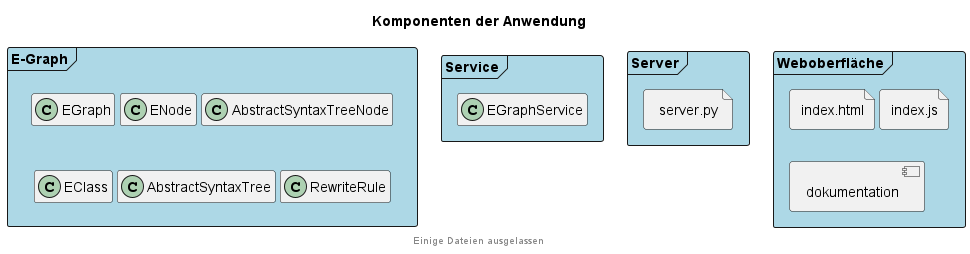
\includegraphics[scale=0.43]{utils/components.png}
        \caption{Architekturdiagramm der Anwendung}
        \label{fig:comps}
    \end{figure}
\end{frame}

\begin{frame}{Ablauf (1)}
    \begin{tcbitemize}[raster equal height=rows, raster columns=3, raster column skip = 1.5cm,
        raster every box/.style={size=small,valign=center,halign=center,colframe=white,colback=white}]
        \tcbitem {\Large $\left(\frac{x \cdot 2}{2} + x \cdot \frac{y - 3 + 3 + z \cdot 0}{x}\right)^2$ }
        \tcbitem \begin{tikzpicture}
            \draw[line width=10mm, -{Stealth[length=4mm, open, round]}, black, thick] (0,0) -- (2,0);
        \end{tikzpicture}
        \tcbitem {\Large $(x + y)^2$ }  
    \end{tcbitemize}\vspace{5mm}
\end{frame}

\begin{frame}{Ablauf (2): AST}
    \begin{figure}[H]
        \centering
        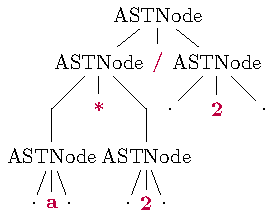
\includegraphics[scale=1.4]{utils/ast.pdf}
        \caption{\textbf{A}bstract \textbf{S}yntax \textbf{T}ree des Teilausdrucks $(x \cdot 2) / 2$}
        \label{fig:komponenten}
    \end{figure}
\end{frame}

\begin{frame}{Ablauf (3): Add}
    %% add - Code
    \begin{columns}[c]
        \column{.6\textwidth}
            
            
        \column{.4\textwidth}
            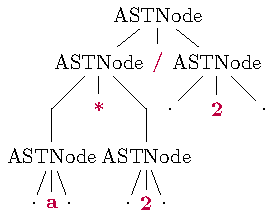
\includegraphics[scale=1]{utils/ast.pdf}
    \end{columns}
\end{frame}

\begin{frame}{Ablauf (4): Saturate}
    %% Eqsat - Code
\end{frame}

\begin{frame}{Ablauf (4): Extract}
    \begin{columns}[c]
        \column{.6\textwidth}
            \textbf{Kostenfunktion}:
            \begin{itemize}
                \item Operatoren: \begin{itemize}
                    \item $+, -, \ll, \gg$: \colorbox{blue-300}{1}
                    \item $*$: \colorbox{blue-300}{2}
                    \item $/$: \colorbox{blue-300}{3}
                \end{itemize}
                \item E-Node ohne Operatoren: \colorbox{blue-300}{0}
                \item E-Node mit Operatoren: \colorbox{blue-300}{Operator + Kosten der Kinder}
                \item E-Class: \colorbox{blue-300}{Kind mit Minimum der Kosten}
            \end{itemize}
            
        \column{.4\textwidth}
            %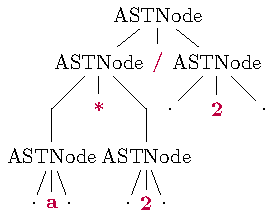
\includegraphics[scale=1]{utils/ast.pdf}
    \end{columns}
\end{frame}